\section{Auswertung}
\label{sec:Auswertung}
\subsection{Bestimmung der Proportionalitätsfaktoren des Torsionsdrahtes}
Zunächst muss die Apparatur vermessen werden.
Die Messergebnisse werden in Tabelle \ref{tab:1} und \ref{tab:2} präsentiert.

\begin{table}[H]
  \centering
  \caption{Radius des Torsionsfadens.}
  \label{tab:1}
  \sisetup{table-format=1.2}
  \begin{tabular}{c}
    \toprule
    {$r [\si{\micro\metre}]$}\\
    \midrule
    \input{build/radius_tabelle.tex}
    \bottomrule
  \end{tabular}
\end{table}

\begin{table}[H]
  \centering
  \caption{Länge des Torsionsfadens oberhalb/unterhalb des Spiegels.}
  \label{tab:2}
  \sisetup{table-format=1.2}
  \begin{tabular}{c c}
    \toprule
    {$L_1 [\si{\centi\metre}]$} & {$L_2 [\si{\centi\metre}]$}\\
    \midrule
    \input{build/laengen_tabelle.tex}
    \bottomrule
  \end{tabular}
\end{table}


Diese Werte werden nun gemittelt, wobei sich der Mittelwert nach
\begin{equation}
  \bar{x} = \frac{1}{n} \sum_{i=1}^n x_i
\end{equation}
und die Standardabweichung nach
\begin{equation}
  S = \sqrt{ \frac{1}{n-1} \sum_{i=1}^n  \bigl(x_i - \bar{x} \bigr)^2  }
\end{equation}
berechnet.
Dementsprechend ergeben sich die gemittelten Apparaturdaten von
\begin{align*}
  L_1 &= \input{build/l1.tex},\\
  L_2 &= \input{build/l2.tex},\\
  r &= \input{build/r.tex}.\\
\end{align*}

Unter Berücksichtigung dieser Daten kann, wie in Kapitel \ref{sec:d1} beschrieben, der Schubmodul bestimmt werden.
Die dazu gemessenen Periodendauern sind in Tabelle \ref{tab:3} dargestellt.

\begin{table}[H]
  \centering
  \caption{Messung der Periodendauer zur Bestimmung des Schubmodules.}
  \label{tab:3}
  \sisetup{table-format=1.2}
  \begin{tabular}{c}
    \toprule
    {$T_1 [\si{\second}]$}\\
    \midrule
    \input{build/a_tabelle.tex}
    \bottomrule
  \end{tabular}
\end{table}

Nach Formel \eqref{eqn:8} aus der Theorie lässt sich somit der Schubmodul errechnen.
Dabei muss neben dem Trägheitsmoment der Kugel, welches sich nach \eqref{eqn:7} berechnet, das Trägheitsmoment der Kugelhalterung berücksichtigt werden, welches dem Versuchsaufbau nach
\begin{align*}
  \theta_{\text{Halterung}} = \SI{22.8}{\gram\centi\metre\squared}
\end{align*}
abgelesen wird.
Mit
\begin{align*}
  \theta = \theta_{\text{Kugel}} + \theta_{\text{Halterung}}
\end{align*}
als Gesamtträgheitsmoment des Aufbaus bestimmt sich das Schubmodul zu
\begin{align*}
  G = 8 \pi \theta \frac{L}{T^2 R^4}.
\end{align*}
Mit dem aus dem Messwerten gemittelten $T$, der Fadenlänge $L_1 + L_2$ sowie dem Versuchsaufbau entnommenen Radius $R$ der Kugel
\begin{align*}
  R = \SI{25.28 +- 0.1}{\milli\metre}
\end{align*}
ergibt sich ein Schubmodul von
\begin{align*}
  G = \input{build/schubmodul.tex}.
\end{align*}
Für die Fehlerrechnung wird bei dieser Rechnung und bei allen folgenden Rechnungen das Gaußsche Fehlerfortpflanzungsgesetz
\begin{equation}
\increment{f} = \sqrt{\Bigl(\frac{\partial f}{\partial x_1}\increment{x_1}\Bigr)^2 + \Bigl(\frac{\partial f}{\partial x_2}\increment{x_2}\Bigr)^2 + \dotsc + \Bigl(\frac{\partial f}{\partial x_n}\increment{x_n}\Bigr)^2}
\end{equation}
für eine Funktion $f(x_1,x_2, \dotsc ,x_n)$, bei der die Größen $x_1, x_2, \dotsc , x_n$ voneinander unabhängig sind, verwendet.
Mit dem vorgegebenen Elastizitätsmodul von
\begin{align*}
  E = \input{build/elastizitaetsmodul.tex}.
\end{align*}
und Formel \eqref{eqn:1} ergibt sich die Poissonsche Querkontraktionszahl zu
\begin{align*}
  \mu = \input{build/querkontraktionszahl.tex}.
\end{align*}
Hieraus folgt zudem aus der Formel \eqref{eqn:2} der Kompressionsmodul zu
\begin{align*}
  Q = \input{build/kompressionsmodul.tex}.
\end{align*}

\subsection{Bestimmung des magnetischen Momentes eines Stabmagneten}
Wie in der Durchführung in Kapitel \ref{sec:d3} beschrieben, soll das magnetische Moment eines in der Kugel verbauten Permamentmagneten bestimmt werden.
Die Ergebnisse für die fünf Messungen sind in Tabelle \ref{tab:4} dargestellt.
\begin{table}[H]
  \centering
  \caption{Periodendauern zur Bestimmung des magnetischen Moments des Permamentmagneten.}
  \label{tab:4}
  \sisetup{table-format=1.2}
  \begin{tabular}{c c c c c}
    \toprule
    {$T_{1} [\si{\second}]$} & {$T_{2} [\si{\second}]$} & {$T_{3} [\si{\second}]$} & {$T_{4} [\si{\second}]$} & {$T_{5} [\si{\second}]$}\\
    \midrule
    \input{build/c_tabelle.tex}
    \midrule
    {$I_1 = \SI{0.2}{\ampere}$} & {$I_2 = \SI{0.4}{\ampere}$} & {$I_3 = \SI{0.6}{\ampere}$} & {$I_4 = \SI{0.8}{\ampere}$} & {$I_5 = \SI{1.0}{\ampere}$} \\
    \bottomrule
  \end{tabular}
\end{table}
Dabei werden die Messungen bei den jeweils dabei angegeben Stromstärke für die Helmholzspulen durchgeführt.
Diese erzeugt bei gegebenen Strom $I$, Windungsanzahl $N$ sowie Spulendurchmesser $R$ ein homogenes Magnetfeld von
\begin{align}
  B = \mu_0 \frac{8 I N}{\sqrt{125} R}.
\end{align}
Die Apparaturwerte werden dem Versuchsaufbau zu
\begin{align*}
  N &= 390 \\
  R &= \SI{78}{\milli\metre}
\end{align*}
entnommen.
Es werden nun die jeweils erzeugten Magnetfelder $B$ gegen den dazugehörigen gemittelten Wert von $T^(-2)$ abgetragen.
Es ergibt sich der in Abbildung \ref{fig:a1} angegebene Plot.

\begin{figure}[H]
  \centering
  \includegraphics{1plot.pdf}
  \caption{Reziproke quadratische Periodendauer in Abhängigkeit vom Magnetfeld.}
  \label{fig:a1}
\end{figure}

Für die daraus folgenden Daten wird ein linearer Fit an die Funktion
\begin{align*}
  y = m x + b
\end{align*}
erstellt.
Dieser wird von SciPy in Python mithilfe der Methode der kleinsten Quadrate durchgeführt.
Es ergeben sich die Parameter
\begin{align*}
  b_{\text{fit}} &= \input{build/bfak_1.tex},\\
  m_{\text{fit}} &= \input{build/propfak_1.tex}.
\end{align*}
Anhand von Gleichung \eqref{eqn:12} lässt sich das magnetische Moment $m$ nun aus dem Fit als
\begin{align}
  m = \frac{4 \pi \theta}{m_{\text{fit}}}
\end{align}
identifizieren, so dass man einen Wert von
\begin{align*}
  m &= \input{build/magnetisches_moment1.tex}
\end{align*}
erhält.

\subsection{Bestimmung der Stärke des Erdmagnetfeldes}
Wie in der Durchführung im Kapitel \ref{sec:d2} beschrieben lässt sich mithilfe des Vorhandenen Aufbaus das Erdmagnetfeld näherungsweise bestimmen.
Die dazu bestimmen Periodendauern sind in Tabelle \ref{tab:5} angegeben.
\begin{table}[H]
  \centering
  \caption{Messung der Periodendauer zur Bestimmung des Erdmagnetfeldes.}
  \label{tab:5}
  \sisetup{table-format=1.2}
  \begin{tabular}{c}
    \toprule
    {$T_1 [\si{\second}]$}\\
    \midrule
    \input{build/b_tabelle.tex}
    \bottomrule
  \end{tabular}
\end{table}
Aus Formel \eqref{eqn:12} folgt dementsprechend das Magnetfeld der Erde zu
\begin{align}
  B = \frac{4 \pi^2 \theta}{T^2 m} - \frac{D}{m}.
\end{align}
Aus den gemittelten Periodendauern sowie unter Kenntnis von $m$, $D$ und $\theta$, welche in den vorherigen Versuchsteilen bestimmt werden, folgt für das Erdmagnetfeld
\begin{align*}
  B_{\text{Erde}} &= \input{build/magnetfeld_erde.tex}.
\end{align*}
%\begin{figure}
%  \centering
%  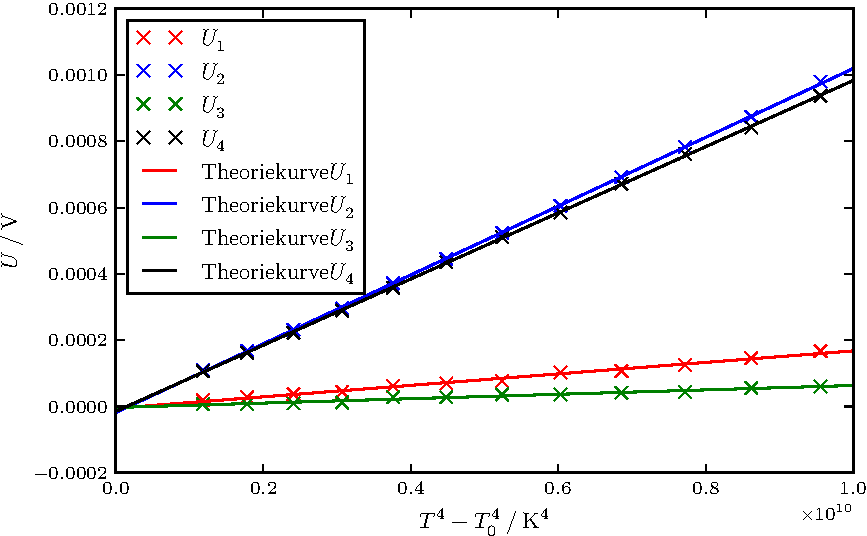
\includegraphics{plot.pdf}
%  \caption{Plot.}
%  \label{fig:plot}
%\end{figure}
%
%\begin{table}
%  \centering
%  \caption{Beispieltabelle}
%  \label{tab:tabelle_beispiel}
%  \sisetup{table-format=1.2}
%  \begin{tabular}{c c}
%    \toprule
%    {$a [\si{\second}]$} & {$b [\si{\kelvin}]$}\\
%    \midrule
%    1.0000  & 11.00 \\
2.0000  & 12.00 \\
3.0000  & 13.00 \\
4.0000  & 14.00 \\
5.0000  & 15.00 \\
6.0000  & 16.00 \\
7.0000  & 17.00 \\
8.0000  & 18.00 \\
9.0000  & 19.00 \\
10.0000 & 20.00 \\

%    \bottomrule
%  \end{tabular}
%\end{table}
%
%Es ergibt sich
%\begin{align}
%  a &= (0 \pm 0) ~ \si{\joule\per\kelvin\per\gram}
 \\
%\end{align}
